%% ----------------------------------------------------------------
%% Conclusion.tex
%% ---------------------------------------------------------------- 
\chapter{Conclusion and Future Work} \label{Chapter: Conclusion}
This thesis aimed to investigate the apple detection problem using the deep learning-based algorithm, RetinaNet. Previous works have repeatedly demonstrated the superiority of deep learning-based methods for agricultural purposes, especially in the field of fruit detection. The biggest advantage of deep learning is that it entirely dismissed feature engineering, which requires expertise from the domain knowledge; thus, it enabled the development of algorithms that apply in universal datasets instead of being crop-specific.

RetinaNet exploits the pyramidal feature hierarchy of the backbone network to build higher-level semantic maps. From each intermediate backbone layer, it obtains feature maps of different spatial sizes, each containing different levels of information. Combination of coarse feature maps rich in information with spatially larger semantically weak maps, results in finer maps, which contain large amounts of information. The resulting feature maps are five pyramidal levels of increasing resolution, each with high content in semantic information, thus enabling detection at multiple scales.

The hyper-parameter tuning is essential for the efficient optimisation of the pipeline. However, in the latest works in the field of fruit detection, hyper-parameter optimisation does not seem that have been analysed in-depth. In the present study, the right predefined anchor boxes' sizes have been efficiently configured through an evolution search algorithm, enabling easier regression. Furthermore, loss function has been modified to adopt more stable values in order to accelerate convergence. Moreover, an analysis between the dataset's annotation size distribution and the predictions' sizes from each pyramidal level of RetinaNet showed, that some layers might be redundant. This observation suggests that different and simpler architectures should be explored. In this way, the present thesis focused on the study of side-network's efficiency through four proposed alternative deployments.

Concerning the network's effectiveness, it was demonstrated that performance scales with the depth of the backbone network; however, that was not the case with the side-network. The lightweight RetinaNet - $\text{C}_\text{i}\text{Reduced}$ consistently performed better compared to more sophisticated architectures. These results suggest that this binary problem is not benefited neither by semantically enriching the feature maps nor by increasing side-network's complexity in a different way.

Surprisingly, an investigation of the performance-training size relationship revealed that even 10 samples are enough for adequate detection. Moreover, maximum performance was achieved by using only 200-500 samples, that is at least 2x times less than the original training set. In this way, growers would be relieved from labelling big datasets. This finding raises questions around the dataset, since it known that the performance of deep learning algorithms scales with the size of the training dataset.

In the last section, optimisation for peak detection demonstrated that, indeed, high resolutions yield better results, but with infinitesimal difference. However, upon increasing resolution the training and inference time increases as well. RetinaNet - $\text{C}_\text{i}\text{Reduced}$ (VGG16) reached its maximum performance with AP=\textbf{0.955} and F1=\textbf{0.908} using a resolution of $800\times1220$, outperforming the state-of-the-art (\cite{bargoti2017deep}). The same model trained on dataset's original resolution ($202\times308$), achieved an AP=\textbf{0.948} and an F1-score=\textbf{0.895} making detections at roughly \textbf{70} FPS, x1.5 times faster than the model of \cite{liang2018apple}. RetinaNet - $\text{C}_\text{i}\text{Reduced}$ is the lightest model with the smallest memory footprint among the rest; it has only 19.8M parameters coupled with VGG16, while VGG19 has 20M parameters itself. Furthermore, the model managed to maintain its first-rate performance even under the more strict $\text{IoU}_{th}$ of 0.5.

Concerning model's limitations, as shown in \sref{nms_threshold}, the detector suppresses detections with overlap $\text{IoU}\geq\text{NMS}_{th}$, as these predictions are registered as multiple detections (Figures \ref{ch6:fig4_2}, \ref{ch6:fig4_3} and \ref{ch5:fig6} demonstrate this behaviour). However, the severity of this problem depends on the context of the application that the framework may be implemented into. For instance, in the case of robotic harvesting it is not crucial, as after a fruit has been gathered, the algorithm can update the detected instances through a new image. On the contrary, in yield estimation applications the model will always undercount, leading in inaccurate results. Furthermore, acquiring data with monocular cameras make the model prone to double-counting, as the model does not identify the objects across frames. As a result, farmers should put extra effort into obtaining datasets with unique instances. Lastly, monocular RGB cameras are incapable of estimating depth; thus the model struggles to distinguish between foreground and background (\fref{ch6:fig3}) resulting in learning spurious rules, such as classifying relevant objects by their relative size.

The ACFR dataset consists of crops of images that span entire trees in an orchard block. The proposed technique can be commercialised through a robotic harvesting application from unmanned ground vehicles, as it allows accurate detections from images captured in relatively short distances. Future work, could involve the exploration of the algorithm's full potential in real-time detection, e.g. in the case of integrating the system on drones, flying between orchard rows. This can be studied through sequential images of entire trees without sub-sampling, in order to investigate if the state-of-the-art performance can be preserved on samples with smaller fruits. Integrating a tracking system on the main pipeline, such as the Hungarian Algorithm, can provide accurate yield mappings.

Finally, concerning the ACFR dataset, RetinaNet achieved similar performance with previous studies in apple detection, through the same dataset in terms of F1-score. In \sref{size_relation}, it was observed that state-of-the-art F1-score reached its peak already from the first 500 samples. This observation combined with several dubious truth annotations, as seen in \fref{ch6:fig4_2}, advocates the reexamination of the ACFR dataset in terms of more reliable ground truth annotations.


 \begin{figure}[!ht]
  \centering
  \subfigure[]{
    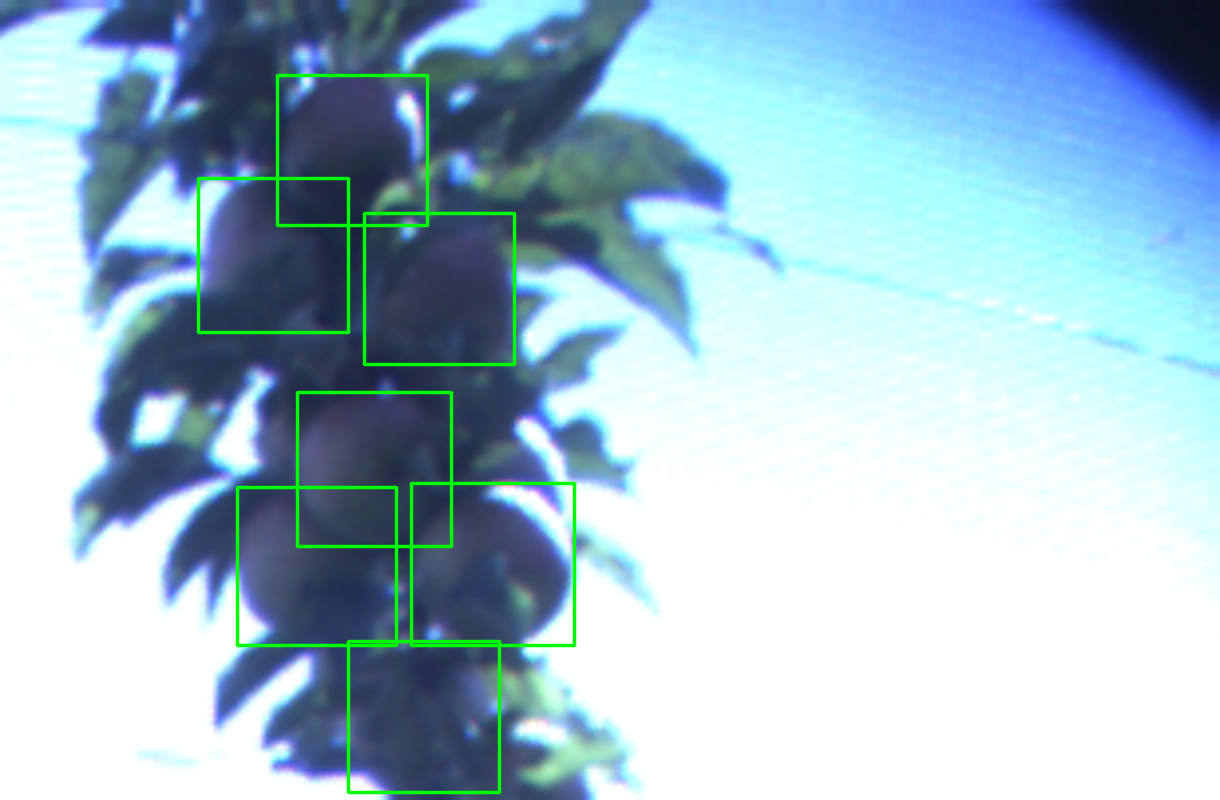
\includegraphics[width=0.31\textwidth]{figures/ch6/fig1_1.png}
    \label{ch6:fig1_1}
  }
  \subfigure[]{
    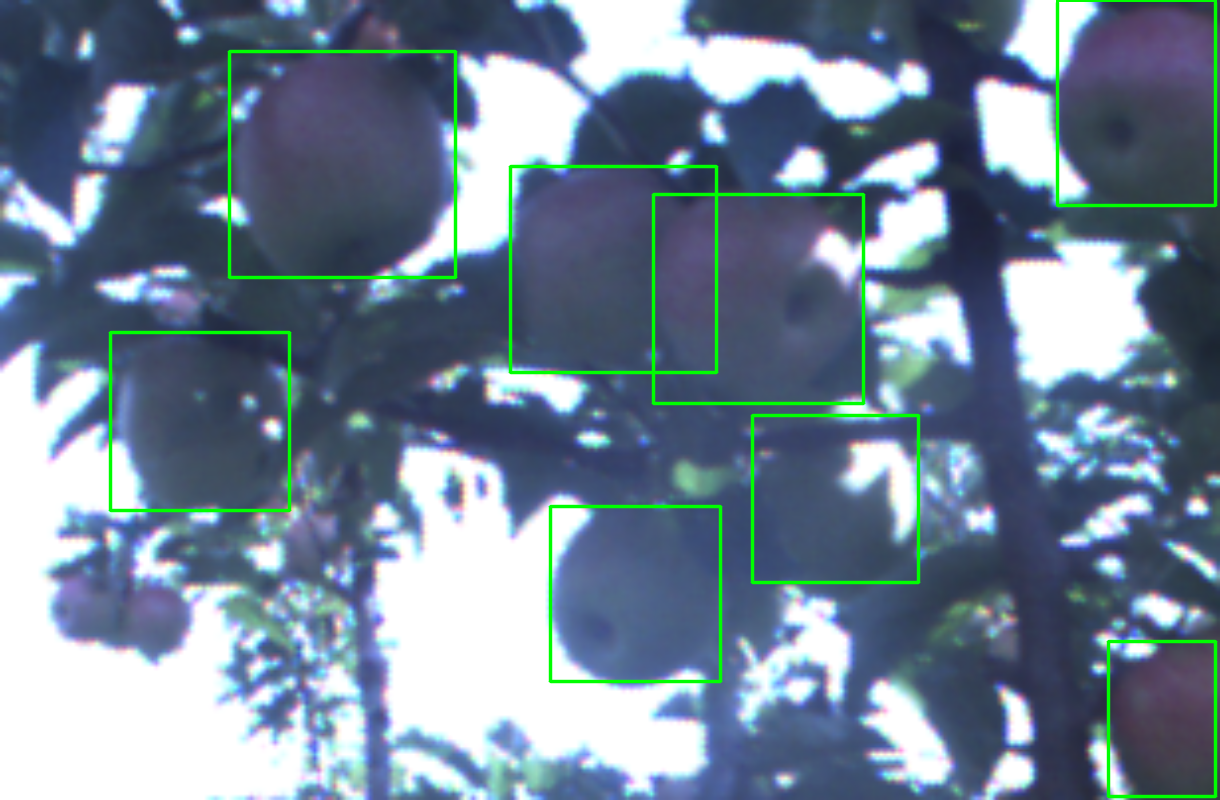
\includegraphics[width=0.31\textwidth]{figures/ch6/fig1_2.png}
    \label{ch6:fig1_2}
  }
  \subfigure[]{
    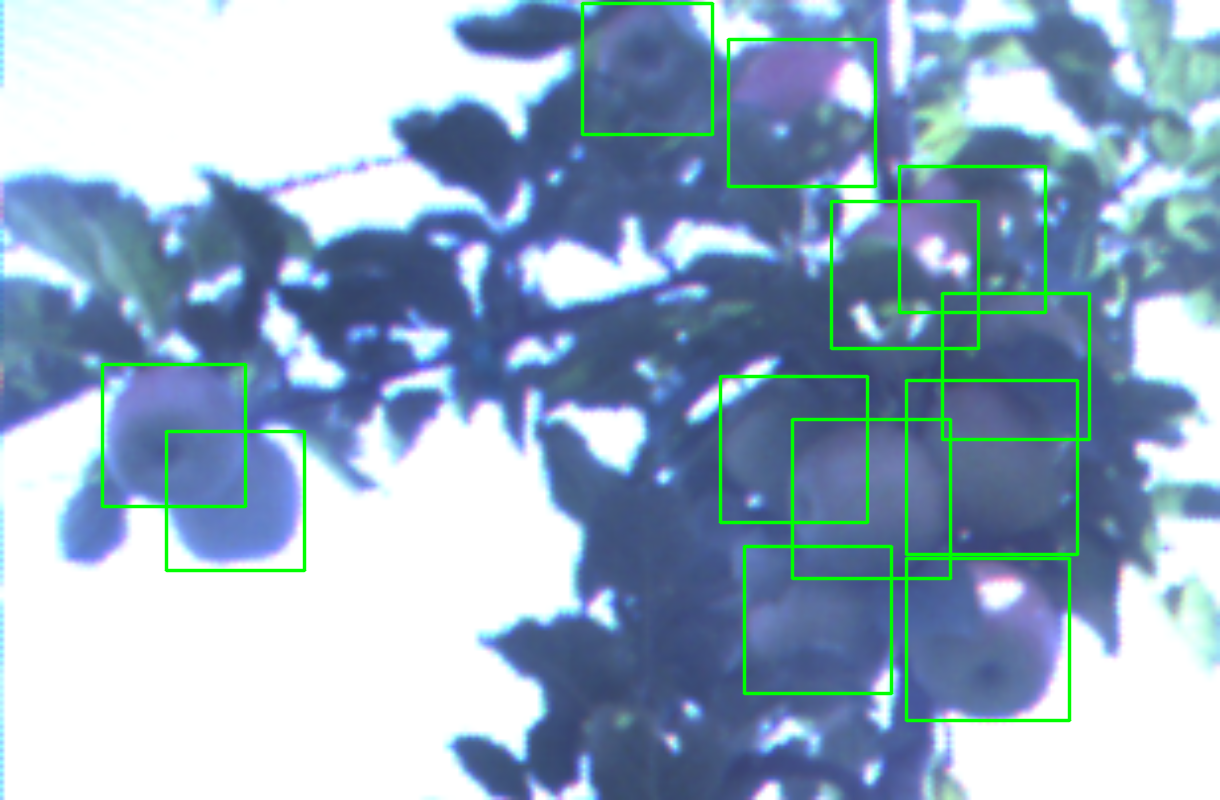
\includegraphics[width=0.31\textwidth]{figures/ch6/fig1_3.png}
    \label{ch6:fig1_3}
  }
  \caption{Cases of successful predictions: (a) in a tight fruit cluster, (b) between foreground and background fruits (bottom-left) and (c) in a fruit cluster with highly occluded instances. Green boxes represent true positive examples.}
  \label{ch6:fig1}

  \subfigure[]{
    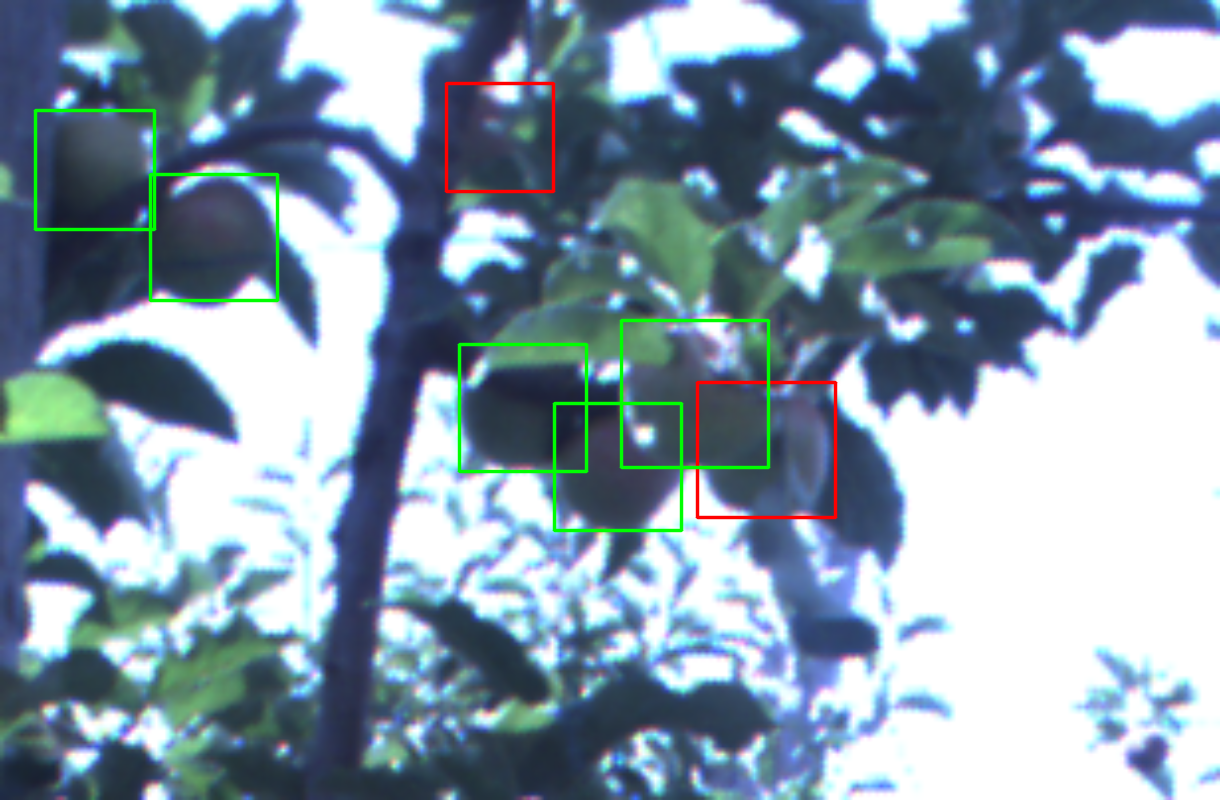
\includegraphics[width=0.31\textwidth]{figures/ch6/fig2_1.png}
    \label{ch6:fig2_1}
  }
  \subfigure[]{
    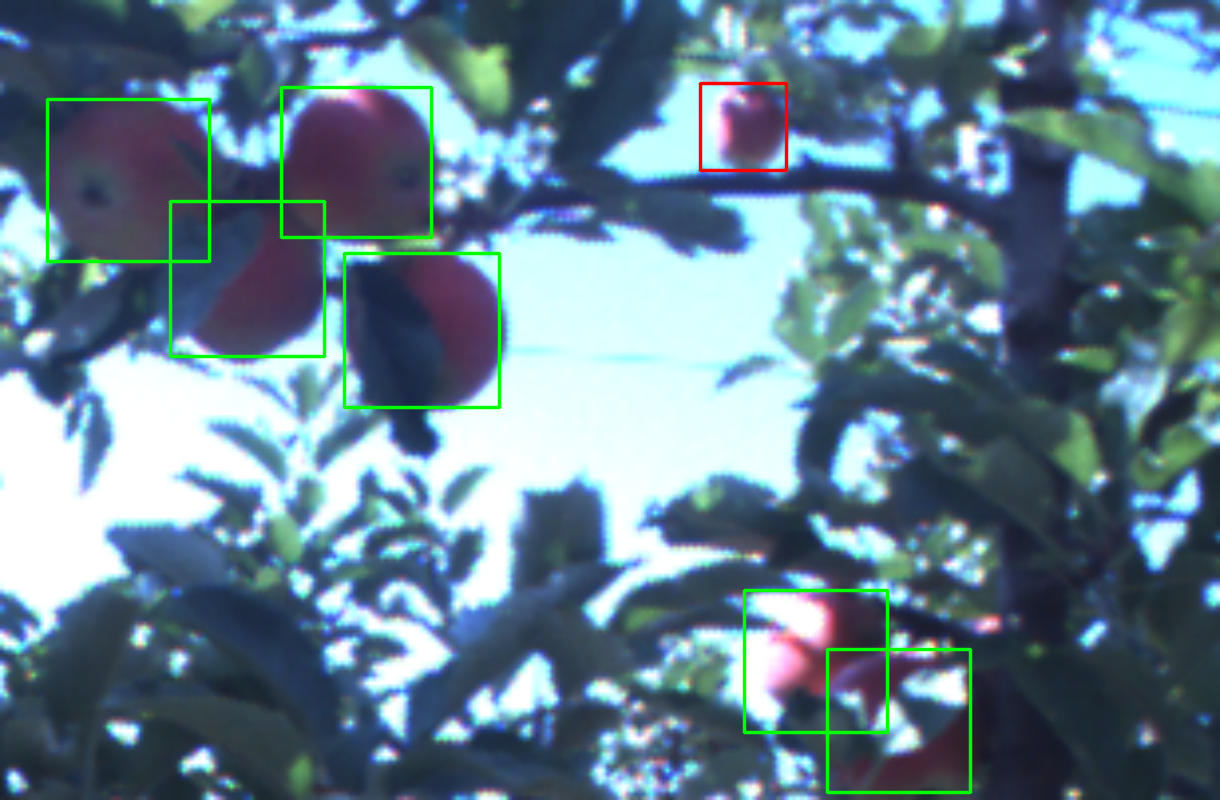
\includegraphics[width=0.31\textwidth]{figures/ch6/fig2_2.png}
    \label{ch6:fig2_2}
  }
  \subfigure[]{
    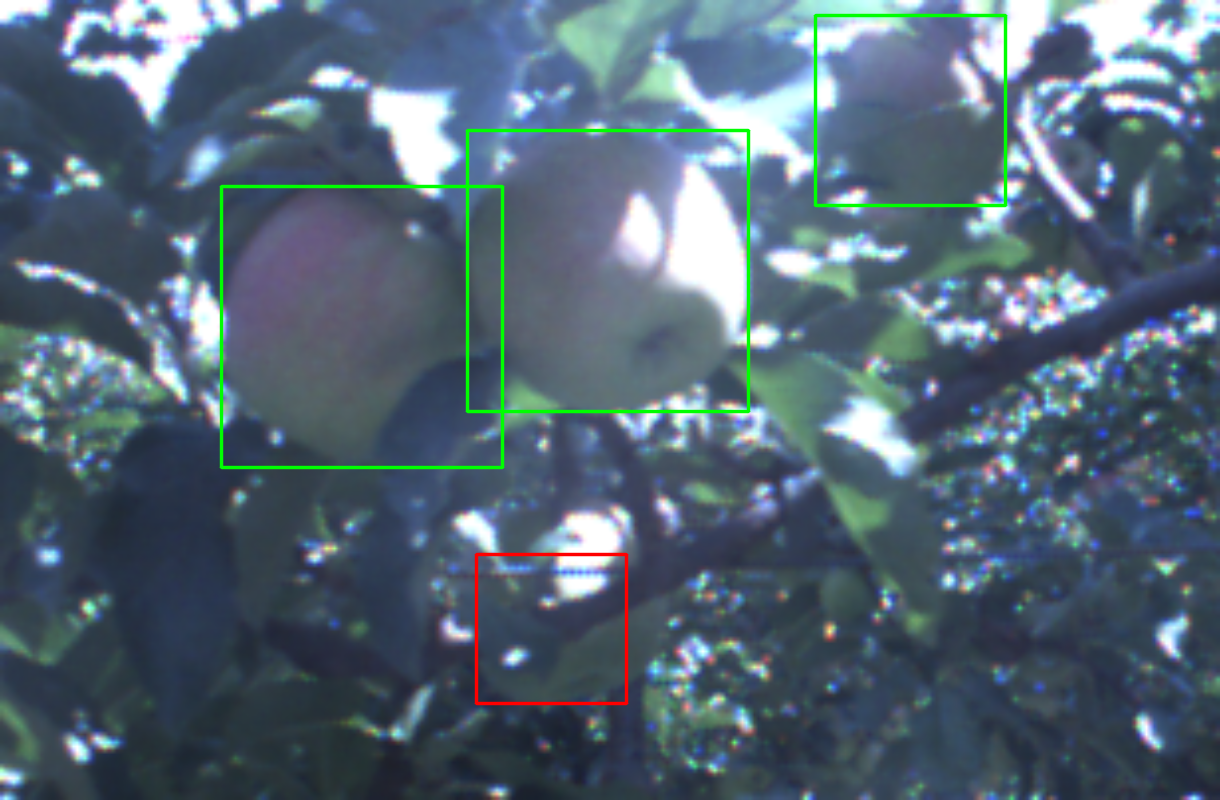
\includegraphics[width=0.31\textwidth]{figures/ch6/fig2_3.png}
    \label{ch6:fig2_3}
  }
  \caption{Error cases where apparently correct predictions are registered as false positives due to lack of annotation. Green and red boxes represent true and false positives respectively.}
  \label{ch6:fig2}

  \subfigure[]{
    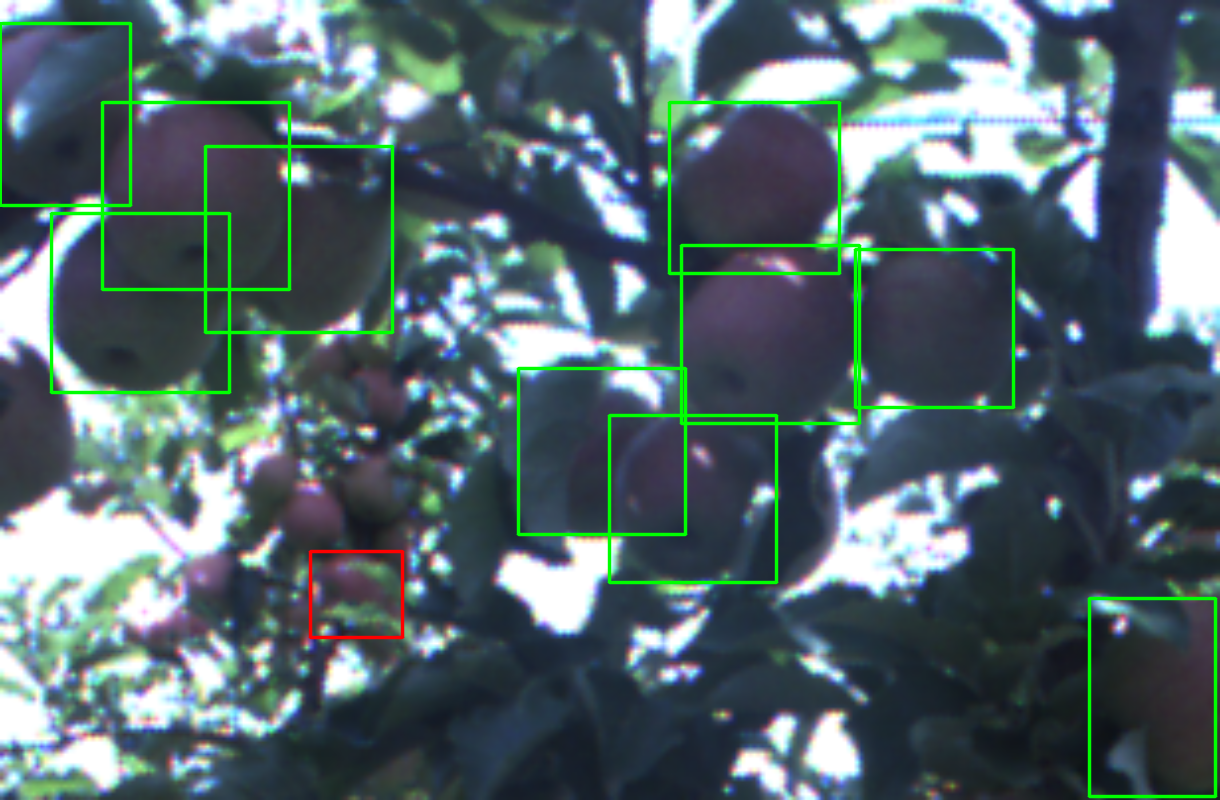
\includegraphics[width=0.31\textwidth]{figures/ch6/fig3_1.png}
    \label{ch6:fig3_1}
  }
  \subfigure[]{
    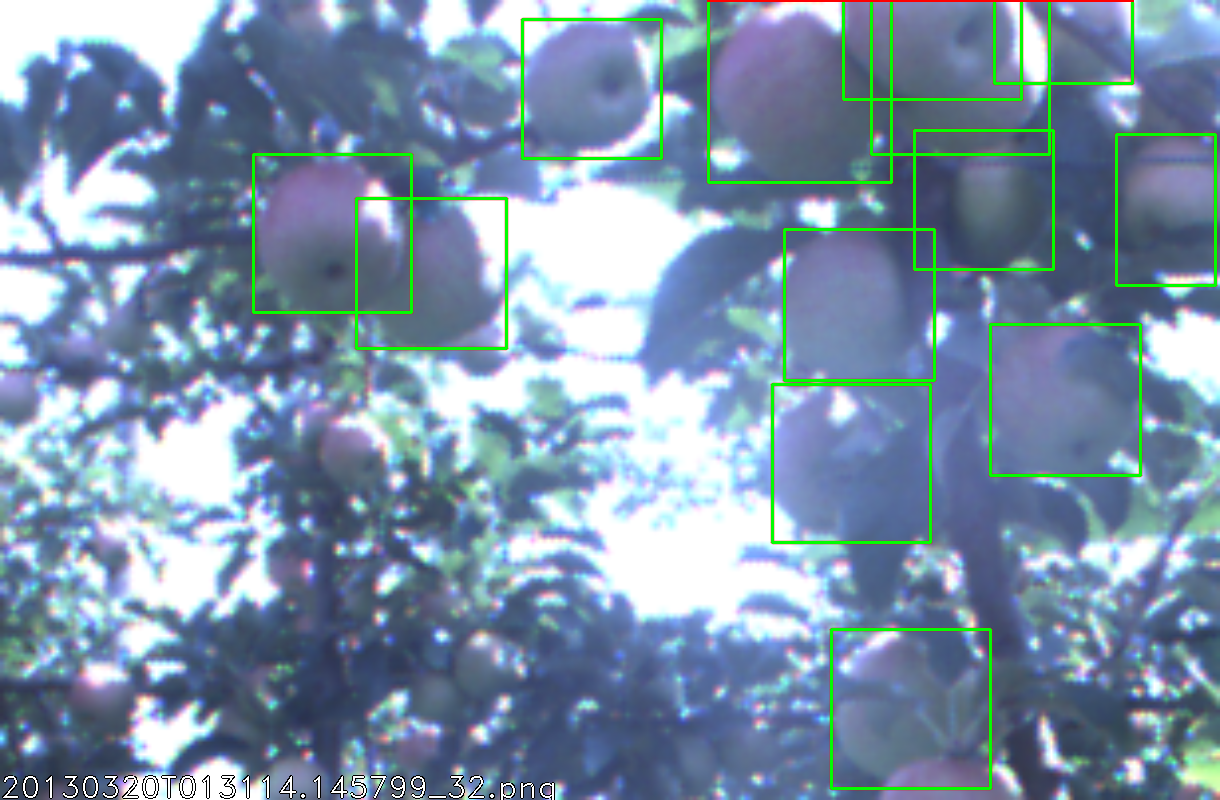
\includegraphics[width=0.31\textwidth]{figures/ch6/fig3_2.png}
    \label{ch6:fig3_2}
  }
  \subfigure[]{
    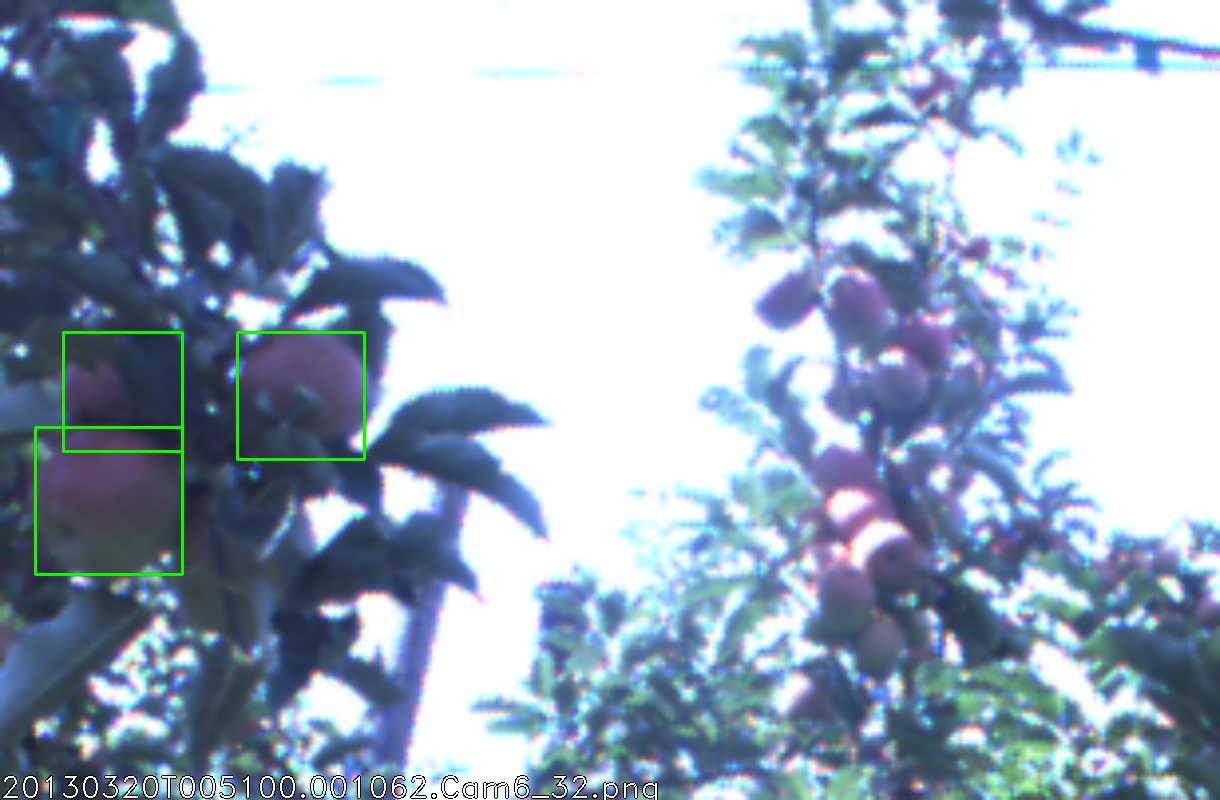
\includegraphics[width=0.31\textwidth]{figures/ch6/fig3_3.png}
    \label{ch6:fig3_3}
  }
  \caption{Some correctly classified hard examples in the training dataset; however, it is disputed if classification to foreground and background was done by fruits' relative size. The model encounters difficulties identifying relevant samples between foreground and background. If the model associates foreground with the relative fruit size, this misleading rule indicates overfitting, as it does not apply in general. Green and red boxes represent true and false positives respectively.}
  \label{ch6:fig3}

  \subfigure[]{
    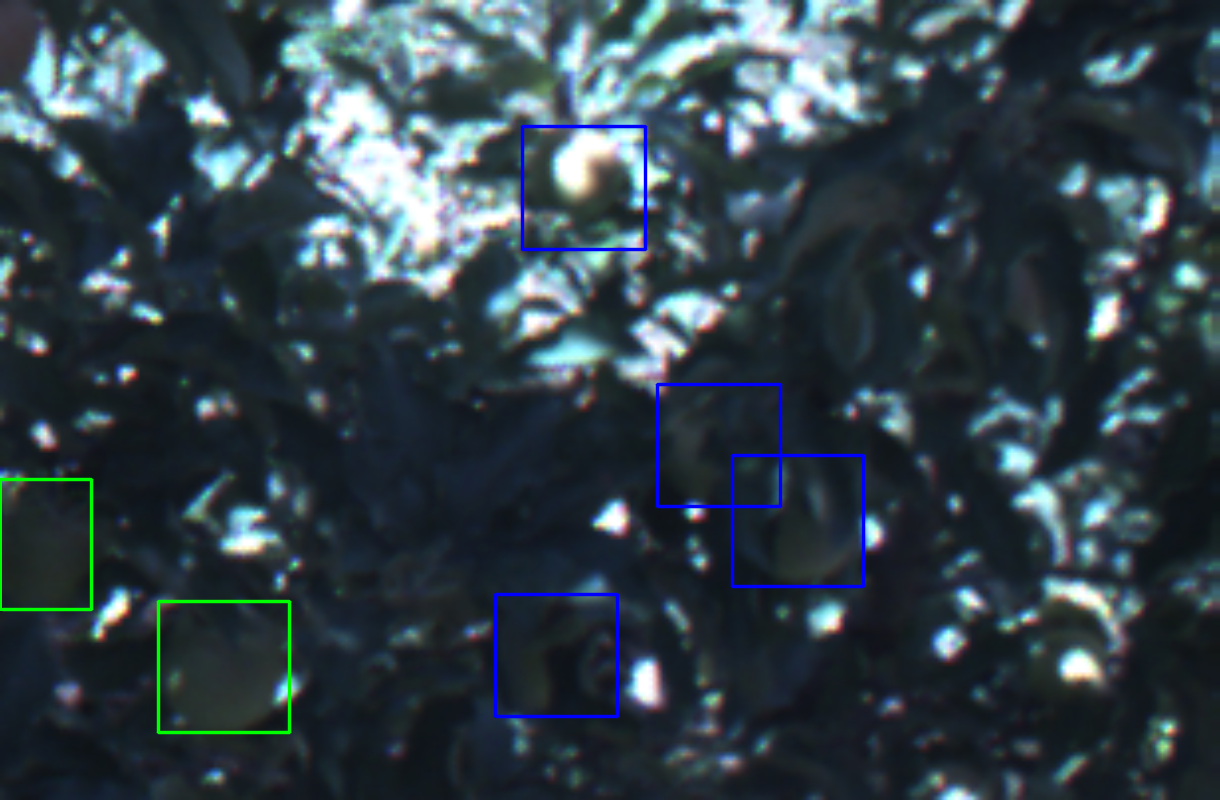
\includegraphics[width=0.31\textwidth]{figures/ch6/fig4_1.png}
    \label{ch6:fig4_1}
  }
  \subfigure[]{
    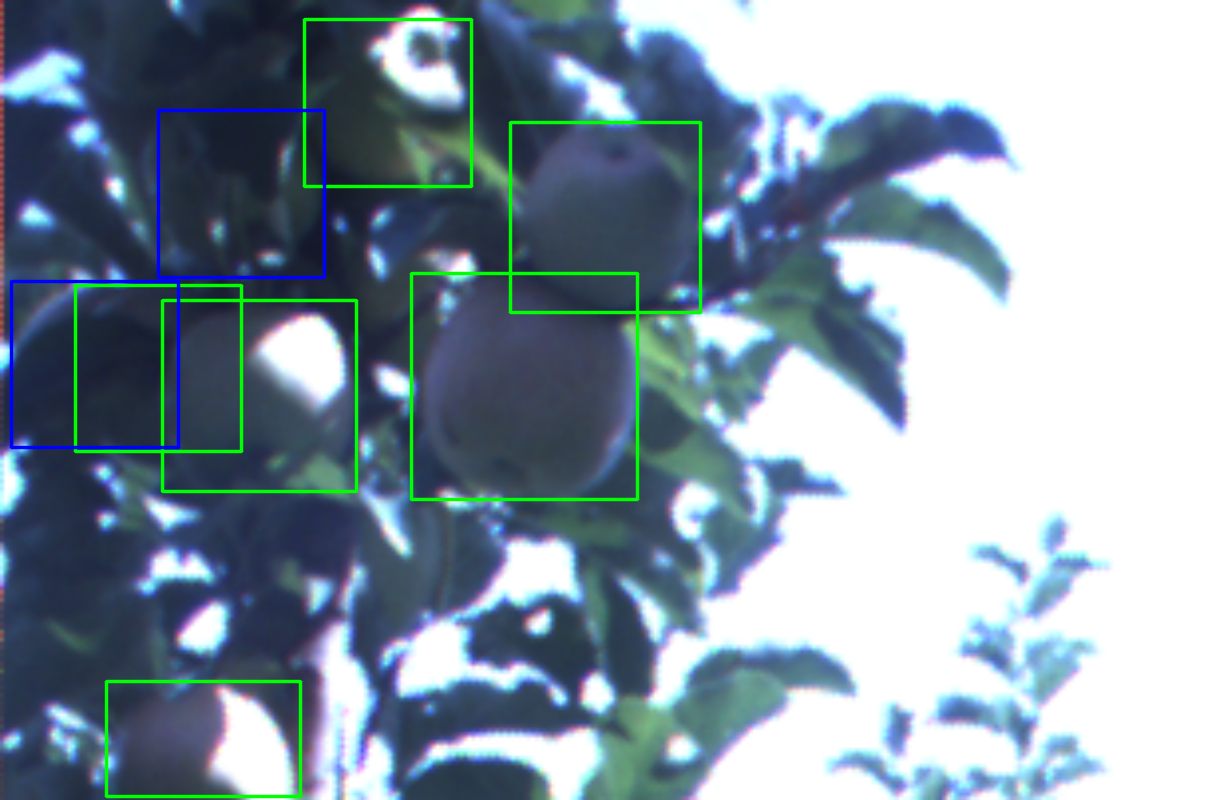
\includegraphics[width=0.31\textwidth]{figures/ch6/fig4_2.png}
    \label{ch6:fig4_2}
  }
  \subfigure[]{
    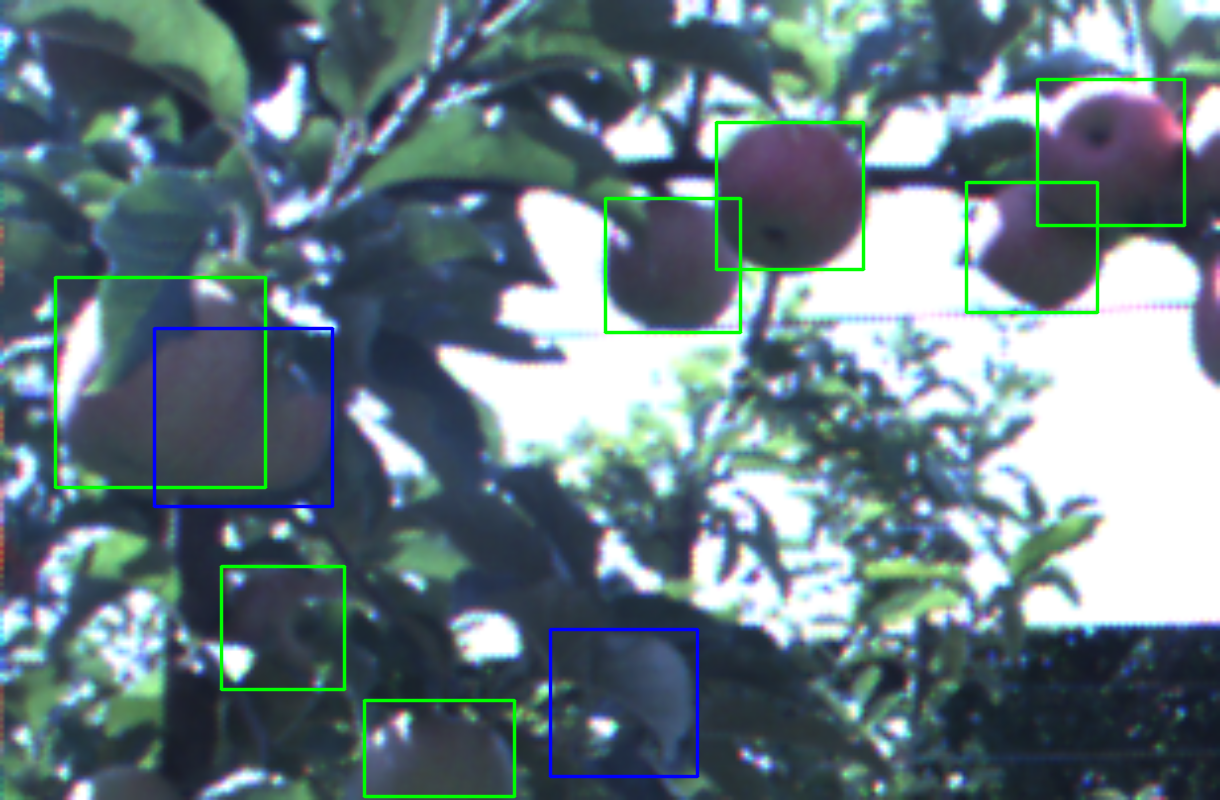
\includegraphics[width=0.31\textwidth]{figures/ch6/fig4_3.png}
    \label{ch6:fig4_3}
  }
  \caption{Interesting false negative predictions from the testing dataset. Errors due to: (a) illumination conditions, (b-c) dubious ground truths. In (b-c), it can be seen that occluded instances with $\text{IoU} \geq \text{NMS}_{th}$ are suppressed to avoid multiple detections of the same object. Green and blue boxes represent true positives and false negatives respectively.}
  \label{ch6:fig4}
\end{figure}

